\begin{figure}[H]
	\centering
	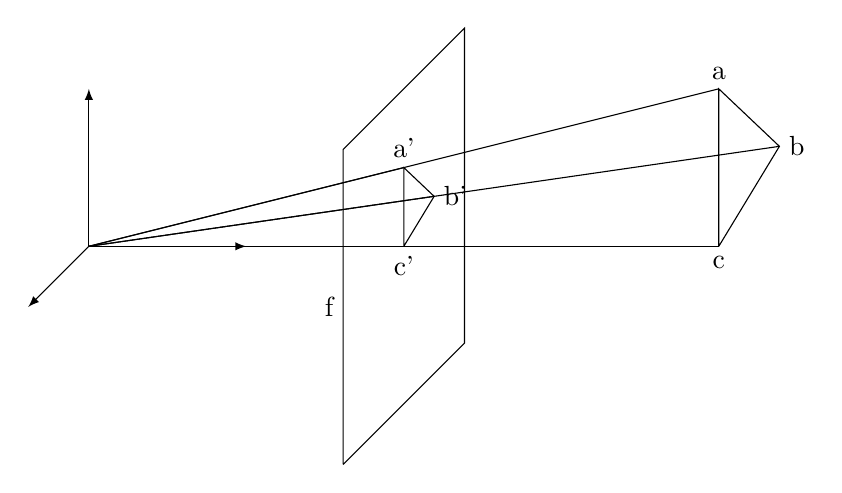
\begin{tikzpicture}[scale=2]
	\draw[-latex] (0,0,0) -- (0,0,1);
	\draw[-latex] (0,0,0) -- (0,1,0);
	\draw[-latex] (0,0,0) -- (1,0,0);
	\node at (0.15,0,0) {\scalebox{2}{$\varangle$}};
	\draw (2,-1,1) -- (2,-1,-1) -- (2,1,-1) -- (2,1,1) -- (2,-1,1) node[, pos=.5, left] {f};
	\draw (0,0,0) -- (4,0,0) node[below] {c};
	\draw (0,0,0) -- (4,1,0) node[above] {a};
	\draw (0,0,0) -- (4,.25,-1) node[right] {b};
	\draw (0,0,0) -- (2,0,0) node[below] {c'};
	\draw (0,0,0) -- (2,.5,0) node[above] {a'};
	\draw (0,0,0) -- (2,.125,-.5) node[right] {b'};
	\draw (4,0,0) -- (4,1,0) -- (4,.25,-1) -- (4,0,0);
	\draw (2,0,0) -- (2,.5,0) -- (2,.125,-.5) -- (2,0,0);
	\end{tikzpicture}
\end{figure}

\begin{align*}
\text{\underline{Bekannt}} &:& f, a', b', c', \underset{\underset{d_{ab}}{\rotatebox{90}{=}}}{|a-b|}, \underset{\underset{d_{bc}}{\rotatebox{90}{=}}}{|b-c|}, \underset{\underset{d_{ca}}{\rotatebox{90}{=}}}{|c-a|}\\
\text{\underline{Gesucht}}&:&a,b,c
\end{align*}

\[ \hat{a} = \vektor{a_x'\\a_y'\\f}\cdot\frac{1}{\sqrt{a_x'^2+a_y'^2+f^2}},~~|\hat{a}|=1, \begin{array}{ccc}
a&=&\alpha\cdot\hat{a}\\
b&=&\beta\cdot\hat{b}\\
c&=&\gamma\cdot\hat{c}
\end{array} \]

\begin{figure}[H]
	\centering
	\begin{tikzpicture}
		\coordinate (0) at (0,0);
		\coordinate (a) at ($(0,0)!1!35:(1,0)$);
		\coordinate (b) at ($(0,0)!1!5:(1,0)$);
		\draw[-latex] (0)--(a) node[above] {$\hat{a}$};
		\draw[-latex] (0)--(b) node[right] {$\hat{b}$};
		\pic["$\varphi$",draw=black, angle eccentricity=1.2,angle radius=.5cm] {angle=b--0--a};
	\end{tikzpicture}
	\caption*{$\cos \varphi = \hat{a}^T\cdot\hat{b}$}
\end{figure}
\begin{align*}
\tag{1}&&|\alpha\hat{a}-\beta\hat{b}| = d_{ab}&&\\
\tag{2}&&|\beta\hat{b}-\gamma\hat{c}| = d_{bc}&&\\
\tag{3}&&|\gamma\hat{c}-\alpha\hat{a}| = d_{ca}&&
\end{align*}
\begin{align*}
\tag{1} && \left( \alpha\hat{a}-\beta\hat{b} \right)^T \cdot \left( \alpha\hat{a} - \beta\hat{b} \right) = d^2_{ab}&&\\
&&\alpha^2\cancel{\hat{a}^2} - 2\alpha\beta\hat{b}^T\hat{a} + \beta^2\cancel{\hat{b}^2} = d^2_{ab}&&
\end{align*}
\begin{align*}
\Aboxed{x^2+y^2-c\cdot x\cdot y &= d}
\end{align*}
\begin{align*}
&&f(x) & = a_n\cdot x^n + a_{n-1} x^{n-1} + \ldots + a_1 \cdot x + a_0&&\\
&&g(x) & = b_m\cdot x^m + b_{m-1} x^{m-1} + \ldots + b_1 \cdot x + b_0&&\\
\end{align*}
\underline{Gesucht:} $x_0$, so dass $f(x_0) = g(x_0) = 0$
\[
S=
\begin{pmatrix}
a_n & a_{n-1} & \ldots & a_1& a_0 & 0 & \ldots & & 0\tikzmark{m1}\\
0&a_n & a_{n-1} & \ldots & a_1& a_0 & 0 & \ldots & 0\\
 & & \ddots &  &    &   & \ddots & & \\
&  &  & a_n & a_{n-1}& \ldots &    & & a_0\tikzmark{m2}\\
b_n & b_{n-1} & \ldots & b_1& b_0 & 0 & \ldots & & 0\tikzmark{n1}\\
0&b_n & b_{n-1} & \ldots & b_1& b_0 & 0 & \ldots & 0\\
& & \ddots &  &    &   & \ddots & & \\
&  &  & b_n & b_{n-1}& \ldots &    & & b_0\tikzmark{n2} 
\end{pmatrix}
\]
\begin{tikzpicture}[overlay, remember picture,decoration={brace,amplitude=5pt}]
\draw[decorate,thick] ($(m1.north east)+(.2,0)$) -- ($(m2.south east)+(.2,0.2)$)
node [midway,right=5pt] {m-mal};
\draw[decorate,thick] ($(n1.north east)+(.25,-.2)$) -- ($(n2.south east)+(.25,0)$)
node [midway,right=5pt] {n-mal};
\end{tikzpicture}
\[ \text{resultante(f,g,x)} = \det(S) = 0 \Leftrightarrow f,g\text{ haben gemeinsame Nullstelle} \]
\[ w_i \vektor{u_i\\v_i\\1} = p_i' = K\cdot M \cdot p_i ~~~ i = 0,\ldots,n-1 ~~ M=\left( R|T \right) \in \mathbb{R}^{3\times4}, ~~~ k\in \mathbb{R}^{3\times3} \]
\[ K = \vektor{f&0&0\\0&f&0\\0&0&f} ~~ \hat{p}_i = \vektor{x_i\\y_i\\z_i} \]
\[ Kp_i = \sum_{j=0}^{3}\alpha_{ij}Kp_j \]
\[ \hat{p}_i = Mp_i \]
\begin{align*}
\text{\underline{Gegeben}} & : & \left( u_i, v_i \right), K, \alpha_{ij}\\
\text{\underline{Gesucht}} & : & w_i, \hat{p_0},\hat{p_1},\hat{p_2},\hat{p_3}
\end{align*}
\begin{minipage}{.4\textwidth}
	\begin{empheq}[box=\widefbox]{align*}
	w_iu_i&=\sum_{j=0}^{3}\alpha_{ij}f\cdot x_j\\
	w_iv_i&=\sum_{j=0}^{3}\alpha_{ij}f\cdot y_j\\
	w_i&=\sum_{j=0}^{3}\alpha_{ij}\cdot z_j
\end{empheq}
\end{minipage}
\hspace*{-2em}
$\Rightarrow$ 
\hspace*{-2em}
\begin{minipage}{.4\textwidth}
\begin{align*}
	u_i\left( \sum\alpha_{ij}z_j \right) &= \sum\alpha_{ij}fx_j\\
	v_i\left( \sum\alpha_{ij}z_j \right) &= \sum\alpha_{ij}fy_j
\end{align*}
\end{minipage}
\begin{minipage}{.5\textwidth}
	12 Unbekannte\\
	$2n$ \underline{lineare} Gleichungen
\end{minipage}
\pagebreak
\[ 
\vektor{%
	 & & &     & & & \\
	 & & &     & & & \\
	 & & &     & & & \\
	 & & &  A  & & & \\
	 & & &     & & & \\
	 & & &     & & & \\
	 & & &     & & & 
	 } \cdot \vektor{x_0\\y_0\\z_0\\\vdots\\x_3\\y_3\\z_3} = \vektor{0\\0\\0\\ \vdots\\0\\0\\0}
 \]
 \[ A \in \mathbb{R}^{2n\times12} \]
 \[ A = \underset{\underset{\mathbb{R}^{2n\times2n}}{\rotatebox{-90}{$\in$}}}{U} \cdot \underset{\underset{\mathbb{R}^{2n\times12}}{\rotatebox{-90}{$\in$}}}{\lambda} \cdot \underset{\underset{\mathbb{R}^{12\times 12}}{\rotatebox{-90}{$\in$}}}{V^T} \]
 Singulärwertzerlegung
 
 \[ V^Tx = \vektor{0\\0\\0\\\vdots\\1} \Rightarrow x = V\cdot\vektor{0\\0\\\vdots\\1} \]
 \[ x = v_n \]
 \[ |\lambda_1| \geq |\lambda_2| \geq \ldots |\lambda_{12}| \]
 \[ U \Lambda V^T x = 0 \]
 \[ \Lambda \underset{y}{\underbrace{V^T x}} = 0 \]
 \[ \Lambda y = 0 \]
 \[ \begin{pmatrix}
 \lambda_1& & & \\
  &\lambda_2 & &0 \\
  & &\ddots & \\
  0& & &\lambda_{12} \\
 \end{pmatrix} \cdot \vektor{y_1\\\vdots\\ \\ y_{12}} = \vektor{0\\0\\\vdots\\0} \]